\chapter{User documentation}
\label{ch:user}
The ability to improve the scalability, agility, and dependability of applications in cloud environments has led to a rise in the popularity of cloud-native development in recent years. The foundation of this strategy is containerization, which offers a standardized and portable way to package and distribute software.

The industry standard for scaling up containerized application management is Kubernetes, a well-known container orchestration technology. In addition to tools for automating these procedures, it offers a complete set of primitives for deploying, scaling, and managing containerized applications.

For automated web browser testing of online applications, particularly in continuous integration and continuous delivery (CI/CD) pipelines, Selenium, an open-source testing framework, is crucial. In a cloud-native setting, Selenium testing integration with Kubernetes is essential.

This project implements a Go-based Kubernetes operator, a custom controller that extends the Kubernetes API and automates the deployment and management of Selenium tests in a Kubernetes cluster while making it easy to integrate into industry-standard monitoring and alerting chains.

This documentation will cover all operator usage aspects, including installation, configuration, and customization. We will also provide examples of how to use the operator to automate the execution of Selenium tests and how to integrate it with other Kubernetes-native tools and services.

\section{Prerequisites of employing the operator}

The operator is designed to be utilized in Kubernetes clusters of business scale, whether they are hosted on public cloud servers or on-premise servers. Although the operator was designed with performance in mind, neither Kubernetes, Selenium hubs nor Prometheus monitoring stacks are intended for local development; however, they are all necessary to show the project's feasibility. Since this tutorial will show it on a local Kubernetes cluster, be aware that hardware-related issues could occur.

Requirements are the followings:
\begin{itemize}
	\item Kubernetes cluster (minikube in the manual)
	\item Shell environment (Linux/Mac OS or Windows with WSL)
	\item kubectl CLI tool
	\item make CLI tool
	\item selenium test exported to .side format
	\item rented or self-managed Selenium Hub service (moon in the manual) 
	\item operator-managed Prometheus in the Kubernetes cluster (kube-prometheus in the manual)
	\item Helm CLI tool for deploying all the above
\end{itemize}

This manual will demonstrate setting up the following Kubernetes environment before deploying the first automated test:

\begin{figure}[H]
	\centering
	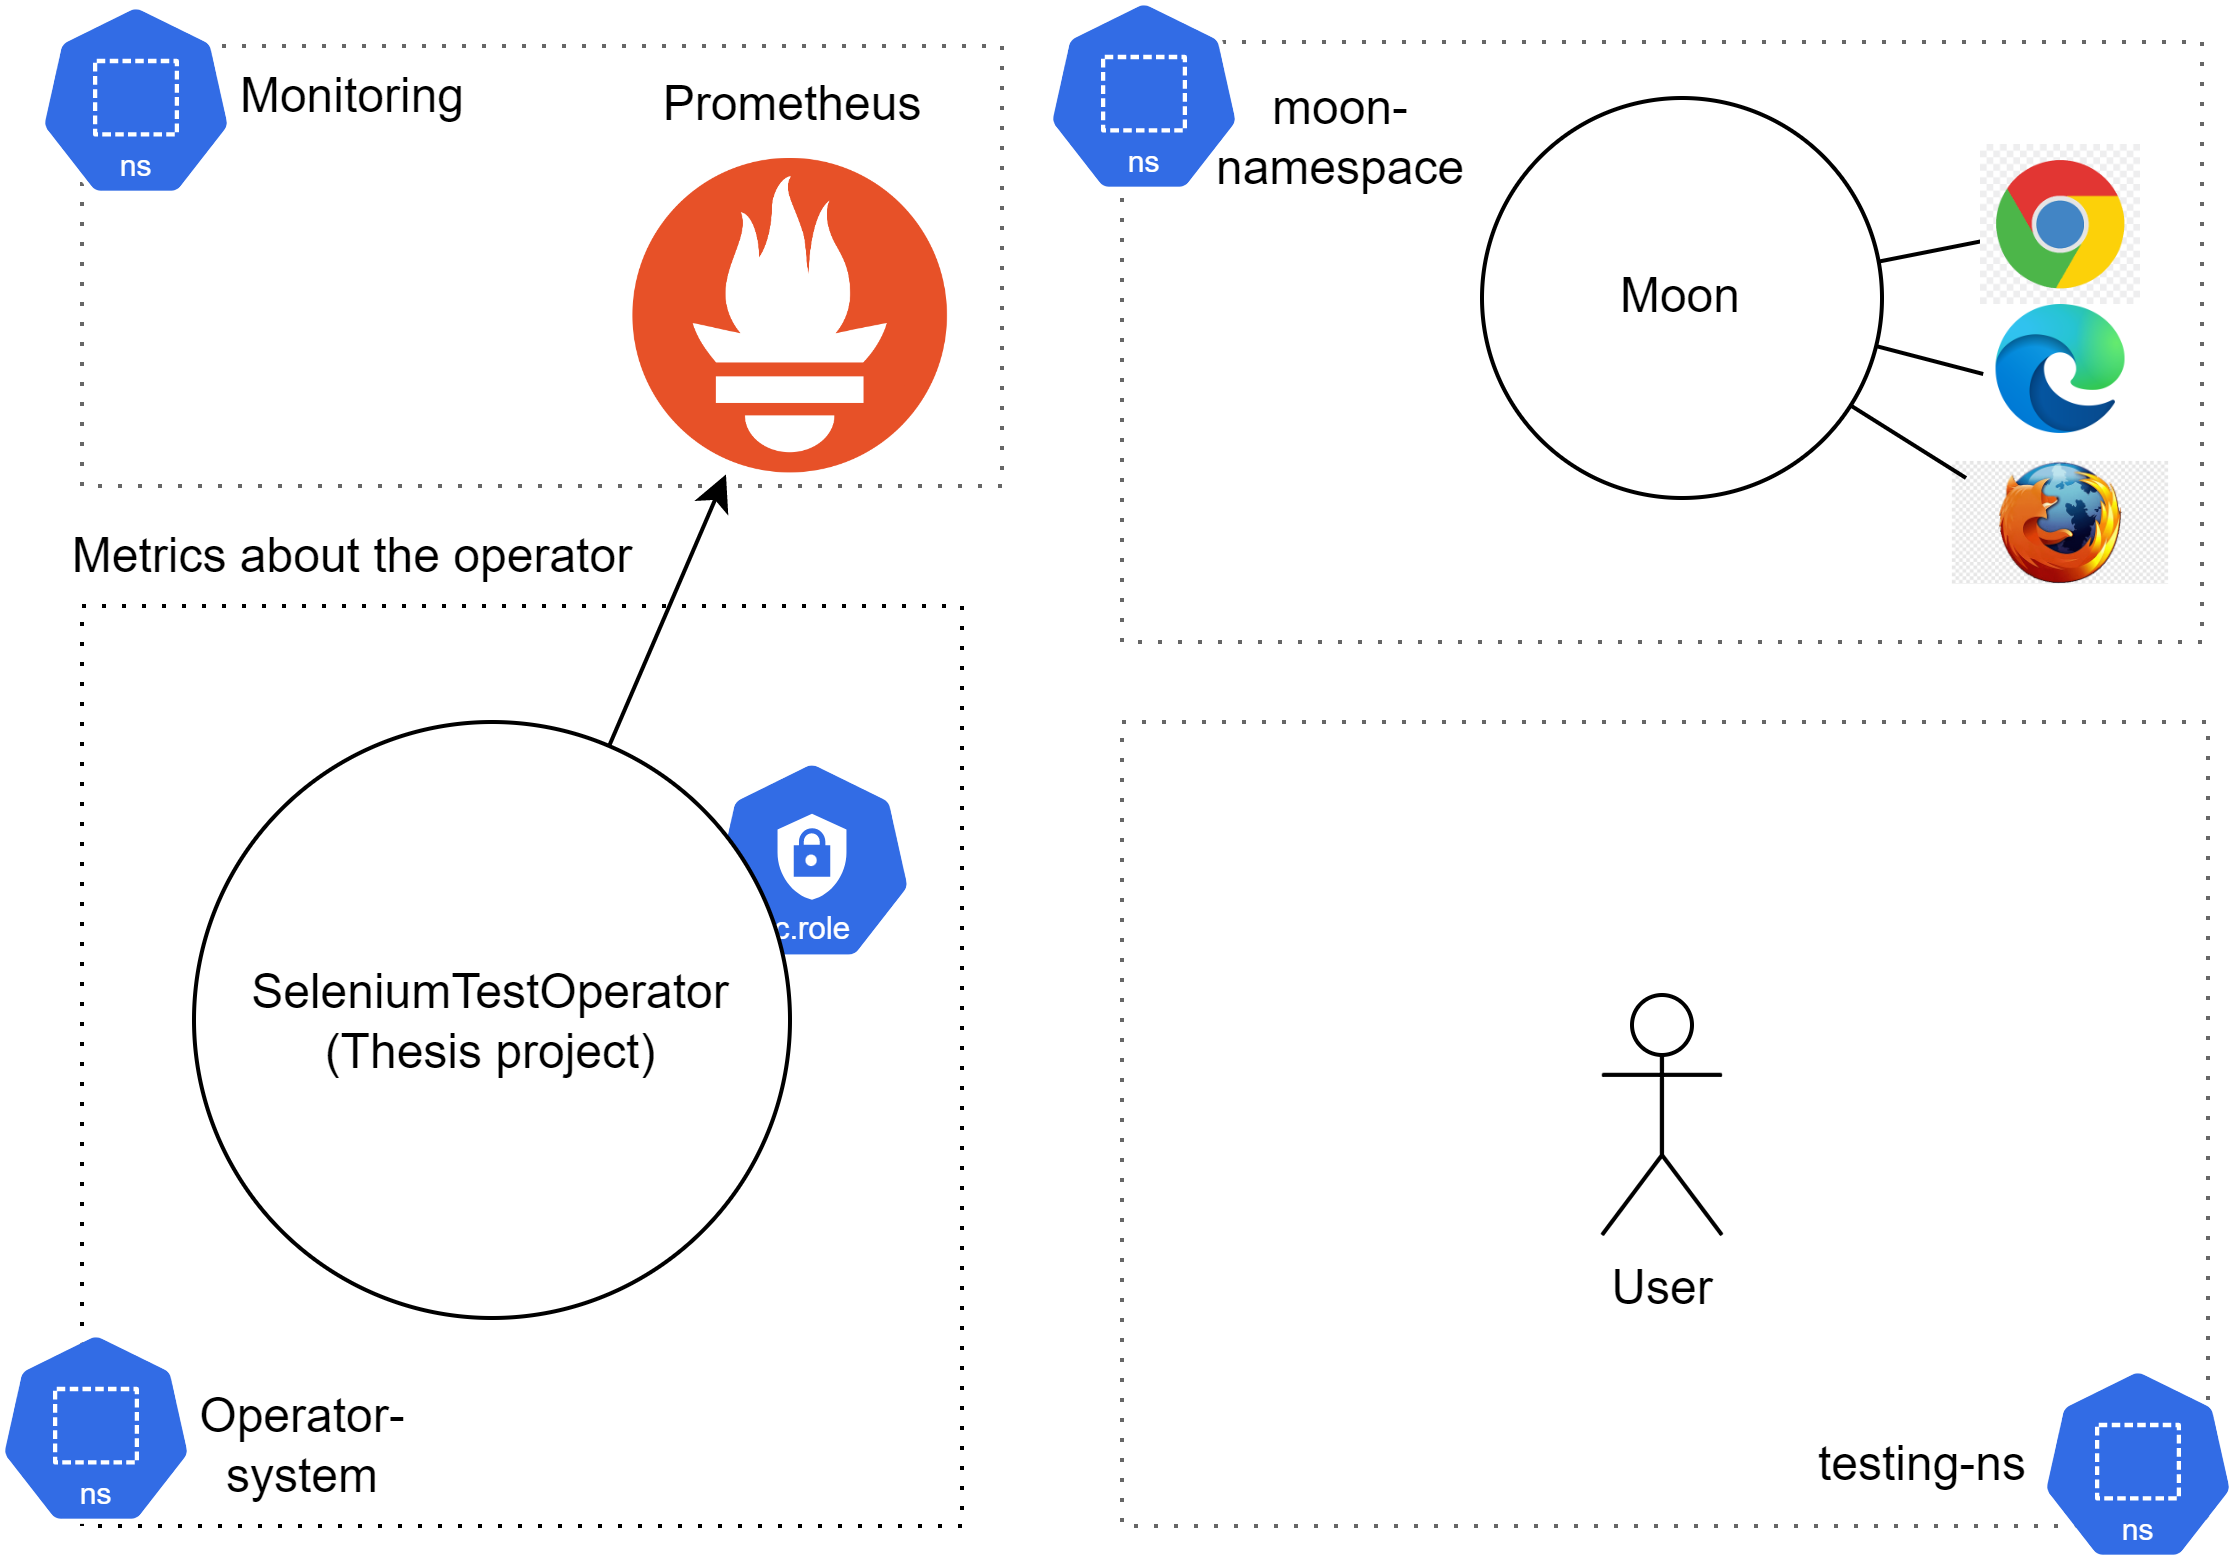
\includegraphics[width=1\textwidth]{before_tests}
	\label{fig:before_tests}
\end{figure}

\subsection{Installing a Minikube cluster}

Before setting up the tools required for running Selenium tests with Kubernetes, a few prerequisites need to be installed. These prerequisites include a Kubernetes cluster, a virtualization tool for Minikube, a shell environment, the kubectl CLI tool, the make CLI tool, and a Selenium test exported to .side format. In this guide, we'll go through each of these prerequisites in detail and show you how to install them on your machine. Once these prerequisites are in place, we can move on to setting up the SeleniumTest Operator and creating custom resources for running Selenium tests.

Before everything else, Windows users has to install WSL by opening the Microsoft Store on Windows and search for "Ubuntu" or any other Linux distribution of choice and launch it.

From now on, shell environment will be used universally between operating systems, meaning shell on either Linux, Mac OS or Windows' WSL.

\begin{itemize}
	\item First of all, intall kubectl:

	\begin{itemize}
		\item In the shell terminal, run the following commands:	
		\begin{lstlisting}[language=bash]
			curl -LO "https://storage.googleapis.com/kubernetes-release/release/$(curl -s https://storage.googleapis.com/kubernetes-release/release/stable.txt)/bin/linux/amd64/kubectl"
			chmod +x ./kubectl
			sudo mv ./kubectl /usr/local/bin/kubectl
		\end{lstlisting}

		\item Verify that kubectl is installed:
		\begin{lstlisting}[language=bash]
			kubectl version --short
		\end{lstlisting}
	\end{itemize}

	\item Secondly, to install make, run the following command in the shell terminal:
	\begin{lstlisting}[language=bash]
		sudo apt-get install build-essential
	\end{lstlisting}
	
	\item Thirdly, to install helm, run In the shell terminal:
	\begin{lstlisting}[language=bash]
		curl -fsSL -o get_helm.sh https://raw.githubusercontent.com/helm/helm/main/scripts/get-helm-3
		chmod 700 get_helm.sh
		./get_helm.sh
	\end{lstlisting}

	\item Fourthly, to install and configure Minikube:

	\begin{itemize}
		\item Windows users:	
		\begin{itemize}
			\item Open your web browser and go to the Minikube releases page on GitHub (https://github.com/kubernetes/minikube/releases).
			\item Find the latest release for Windows and download the executable file (e.g., minikube-windows-amd64.exe).
			\item Move the downloaded executable to a folder that is included in your PATH environment variable. For example, you can move it to the "C:\\Windows\\System32" folder.
			\item Install Docker desktop for Minikube from its offical site: https://www.docker.com/products/docker-desktop/
		\end{itemize}
		\item Linux users:
		\begin{lstlisting}[language=bash]
			curl -LO https://storage.googleapis.com/minikube/releases/latest/minikube-linux-amd64
			sudo install minikube-linux-amd64 /usr/local/bin/minikube
		\end{lstlisting}
		\item Mac users:
		\begin{itemize}
			\item Install Homebrew by running the following command in Terminal:
			\begin{lstlisting}[language=bash]
				/bin/bash -c "$(curl -fsSL https://raw.githubusercontent.com/Homebrew/install/HEAD/install.sh)"
			\end{lstlisting}

			\item Once Homebrew is installed, you can install minikube by running the following command in Terminal:
			\begin{lstlisting}[language=bash]
				brew install minikube
			\end{lstlisting}
		\end{itemize}
		\item After the installation is complete, validate it with the following command:
		\begin{lstlisting}[language=bash]
			minikube version
		\end{lstlisting}	
	\end{itemize}

	\item Lastly, we need to start Minikube:
	\begin{itemize}
		\item Minikube startup under Windows:
		\begin{lstlisting}[language=bash]
			minikube start --cpus=4 --memory=8G --disk-size=30G --driver=docker
		\end{lstlisting}
		\item Minikube startup under MacOS:
		\begin{lstlisting}[language=bash]
			minikube start --cpus=4 --memory=8G --disk-size=20G --driver=hyperkit
		\end{lstlisting}
		\item Minikube startup under MacOS
		\begin{lstlisting}[language=bash]
			minikube start --cpus=4 --memory=8G --disk-size=20G --driver kvm2
		\end{lstlisting}
	\end{itemize}
	\item Even though Moon advises against using Docker as a driver, it is necessary from a networking perspective for Windows users in order to be able to access the cluster from WSL. Providing Minikube with more resources is strongly recommended if possible, but these should be the absolute minimum.
	\item Verify that Minikube is running:
	\begin{lstlisting}[language=bash]
		kubectl cluster-info
	\end{lstlisting}
\end{itemize}

\subsection{Solving kubectl connection problem on Windows}

A configuration file for the kubectl command-line tool for Kubernetes can be found at "~/.kube/config". In addition to the credentials required for cluster authentication, it indicates the Kubernetes cluster with which kubectl should communicate.

Depending on the setup, when installing Minikube, it creates a Kubernetes cluster in a virtual machine or a container. Minikube changes the computer's "~/.kube/config" file to set up kubectl to use this new cluster automatically. As a result, kubectl can communicate with the Minikube cluster.

Windows users encounter a problem since Minikube sets the configuration file at the Windows operating system level, whereas kubectl refers to the configuration file contained in the WSL distribution.

\begin{figure}[H]
	\centering
	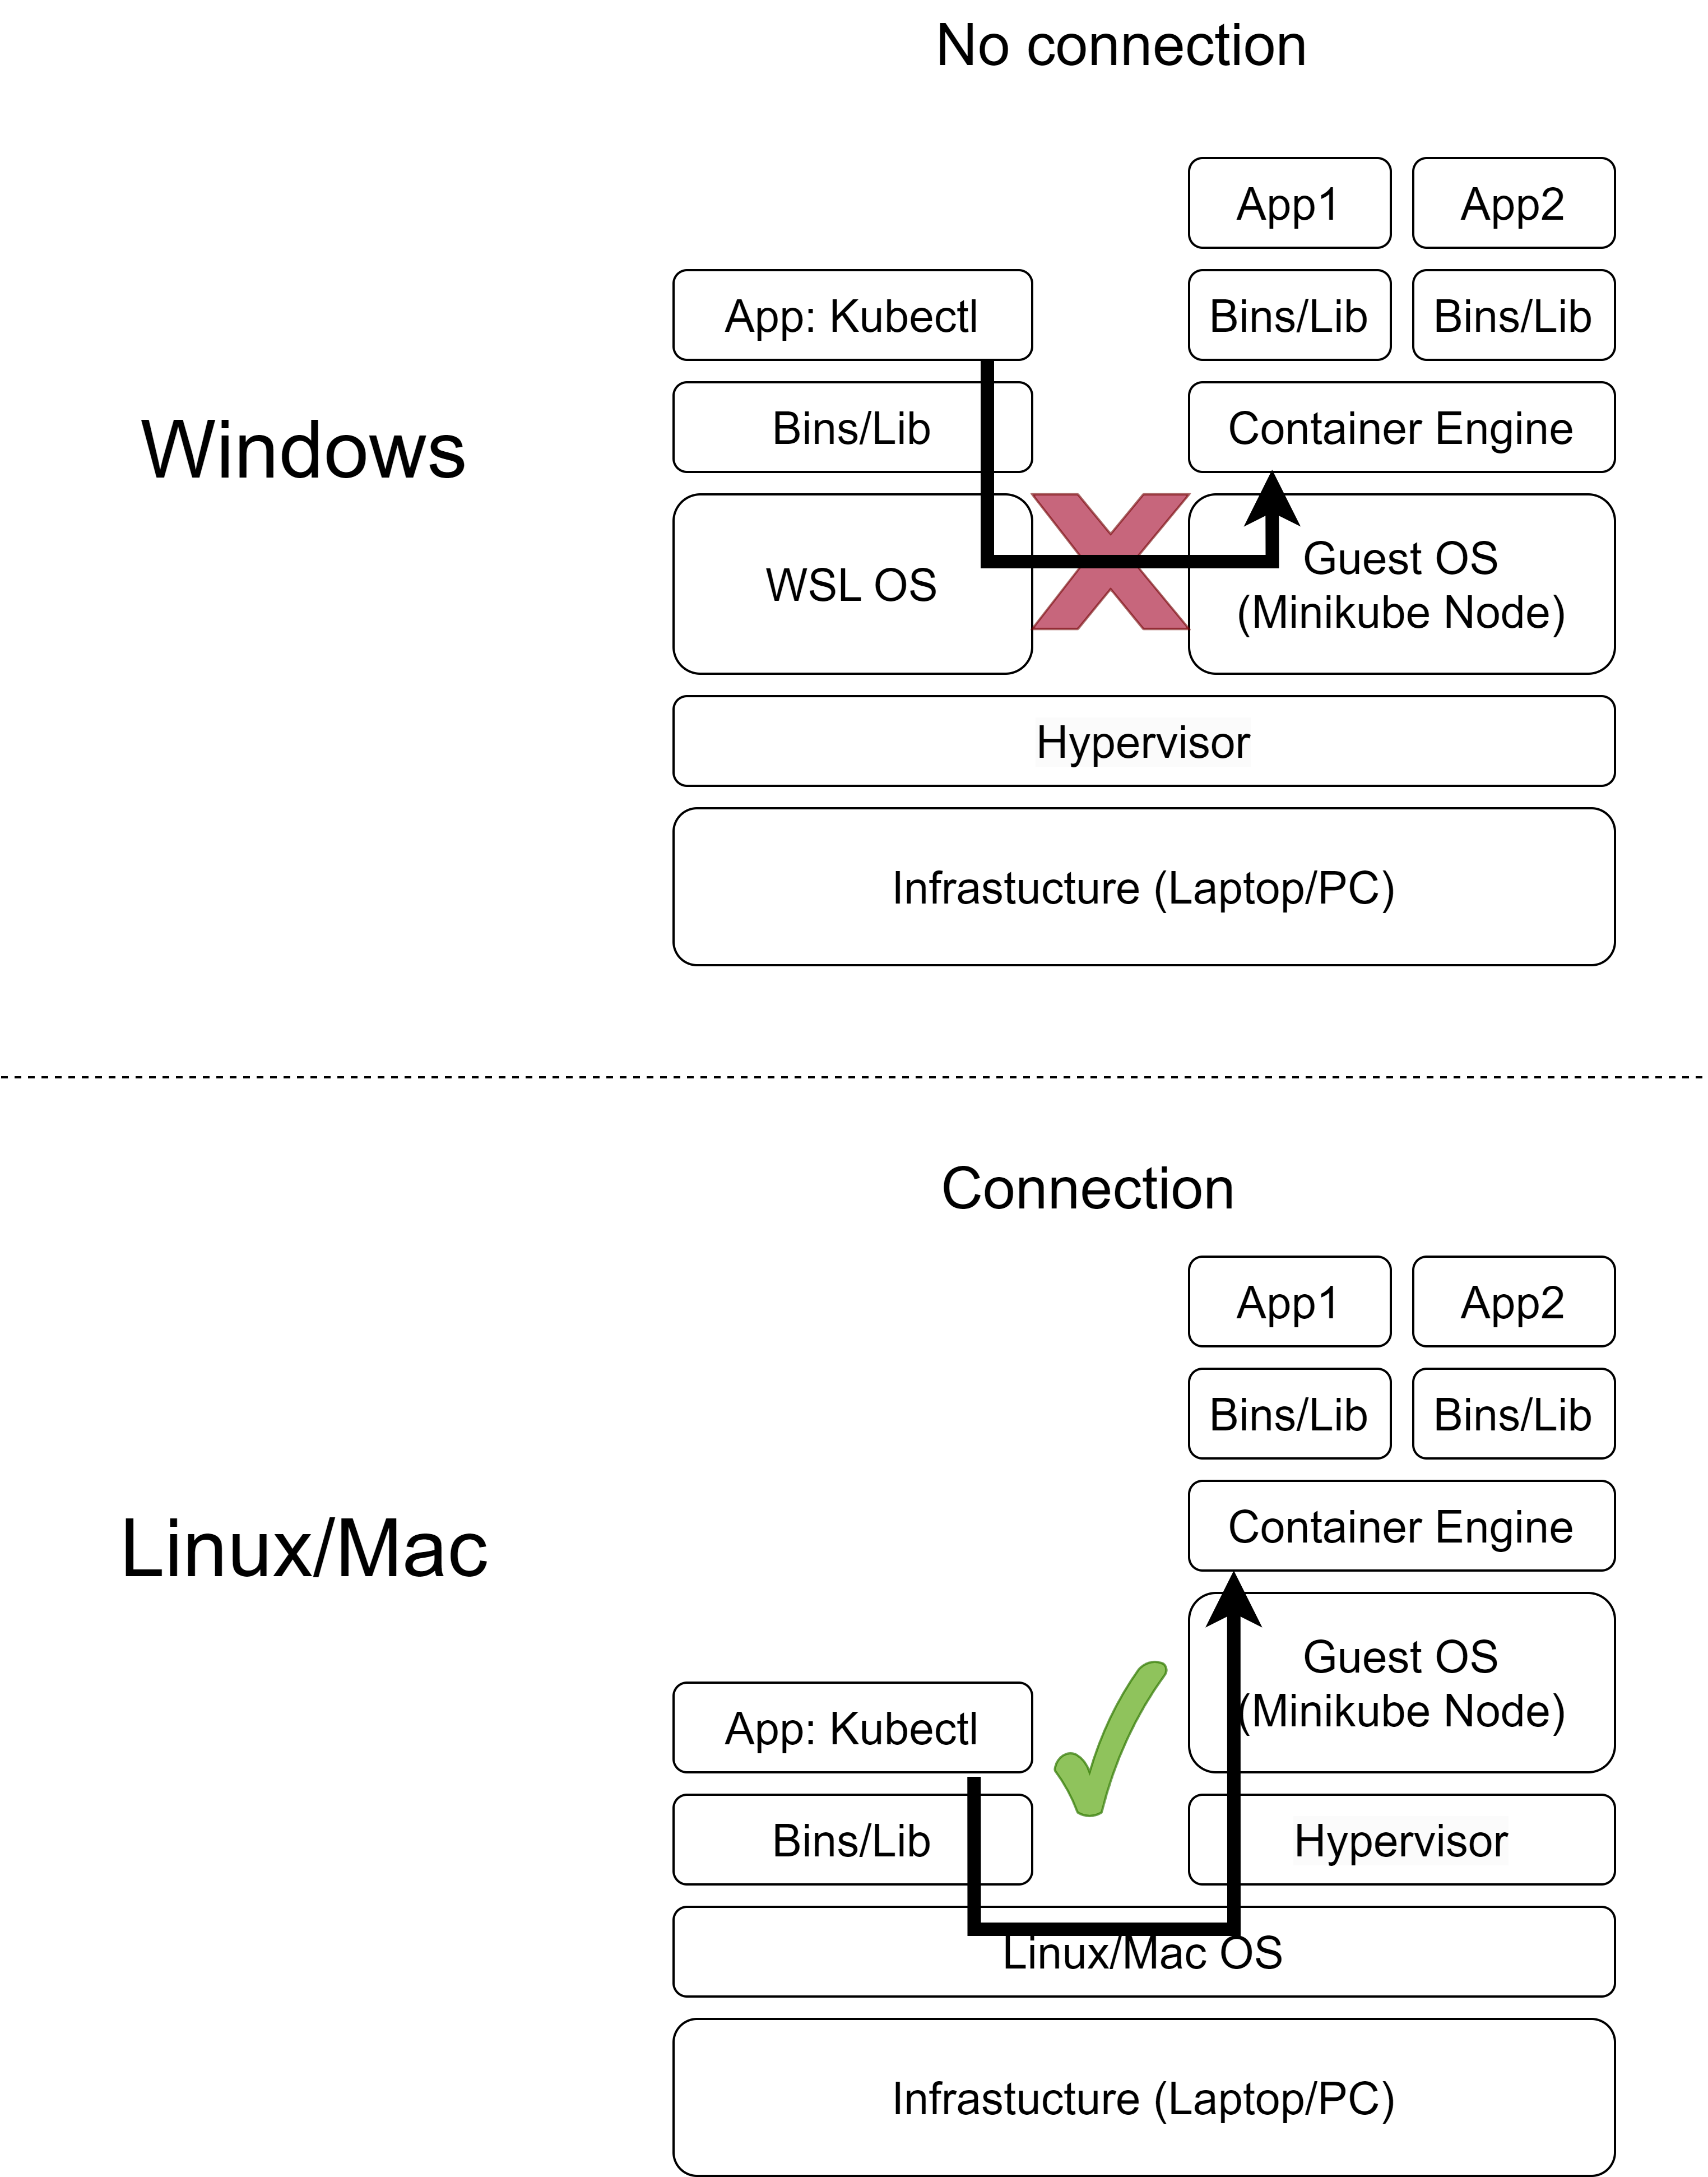
\includegraphics[width=1\textwidth]{window_virtualisation}
	\label{fig:window_virtualisation}
\end{figure}

We must manually generate the kubeconfig file based on the one Minikube created to fix the problem. Although the two files will be very similar, there will be a few minor adjustments because one was created for Windows and the other for Linux.

This is how the new kubeconfig file should appear:

\begin{lstlisting}[language=bash]
	apiVersion: v1
	clusters:
	- cluster:
		certificate-authority: /mnt/c/Users/Your_User/.minikube/ca.crt
		extensions:
		- extension:
			last-update: Sat, 18 Mar 2023 17:26:55 CET
			provider: minikube.sigs.k8s.io
			version: v1.27.0
		  name: cluster_info
		server: https://127.0.0.1:8443
	  name: minikube
	contexts:
	- context:
		cluster: minikube
		extensions:
		- extension:
			last-update: Tue, 02 May 2023 22:28:36 CEST
			provider: minikube.sigs.k8s.io
			version: v1.27.0
		  name: context_info
		namespace: default
		user: minikube
	  name: minikube
	current-context: minikube
	kind: Config
	preferences: {}
	users:
	- name: minikube
	  user:
		client-certificate: /mnt/c/Users/Your_User/.minikube/profiles/minikube/client.crt
		client-key: /mnt/c/Users/Your_User/.minikube/profiles/minikube/client.key
\end{lstlisting}

After creating the file, run the following command in the WSL terminal:
\begin{lstlisting}[language=bash]
	export KUBECONFIG=path/to/your/kubeconfig
\end{lstlisting}

Lastly, verify that Minikube is reachable:
\begin{lstlisting}[language=bash]
	kubectl cluster-info
\end{lstlisting}

\subsection{Deploying the required applications to the cluster}

This section will set up the kube-prometheus, Moon, and seleniumTest operator on our Kubernetes cluster. These tools are essential for testing and monitoring our cluster to ensure it runs smoothly and dependably. For our cluster, kube-prometheus offers a reliable monitoring solution that enables us to keep an eye on critical parameters like resource utilization and application performance. While the SeleniumTest Operator automates the deployment and upkeep of those tests in our Kubernetes cluster, Moon is a Selenium Grid implementation that we will use to run our Selenium tests. 

We will only deploy the Prometheus operator portion of the kube-prometheus stack because of the limited hardware resources available locally, as the other components are useless for this demonstration. Enter the operator repository to get started, then execute the following commands:
\begin{lstlisting}[language=bash]
	kubectl apply --server-side -f prometheus/setup
	kubectl wait --for condition=Established --all CustomResourceDefinition --namespace=monitoring
	kubectl apply -f prometheus/
\end{lstlisting}

Whenever there are issues, visit kube-prometheus's official github page for more details on how to deploy it: https://github.com/prometheus-operator/kube-prometheus

The following commands will deploy Moon, the Selenium Grid implementation, so that the tests may be run:
\begin{lstlisting}[language=bash]
	helm repo add aerokube https://charts.aerokube.com/
	helm repo update
	kubectl create namespace moon
	helm upgrade --install -f moon_values.yaml -n moon moon aerokube/moon2
\end{lstlisting}
Ingress controller is disabled in the moon_values.yaml file because we won't attempt to contact Moon from outside the cluster.

The seleniumTest operator can then be deployed; perform the following steps from the operator's repository:
\begin{lstlisting}[language=bash]
	make deploy IMG=quay.io/molnar_liviusz/selenium-test-operator:v0.0.24
\end{lstlisting}

Finally, we need to create and change the context to the namespace for our project, where we will launch all of the Selenium tests:
\begin{lstlisting}[language=bash]
	kubectl create namespace testing-ns
	kubectl config set-context --current --namespace=testing-ns
\end{lstlisting}

Downloading Lens is advised for simpler cluster management (https://k8slens.dev/). Lens offers a straightforward and understandable graphical user interface for controlling Kubernetes clusters. Users can navigate and change resources, view their cluster's current state, and keep an eye on performance indicators in real time. Additionally, Lens supports numerous clusters and offers a single location for managing them all. Lens is a fantastic alternative for developers and system administrators who need to work with Kubernetes on a regular basis due to its user-friendly interface and extensive feature set.

The outcome of all this is that we now have our cluster configured, achieving the cluster state shown in the previous architecture diagram, with the seleniumTest operator, Prometheus, to query our operator's metrics (including the test results), and Moon deployment as a Selenium Grid implementation. The test recordings are the final component needed to deploy tests.

\subsection{Recorded selenium tests with Selenium IDE}

Selenium IDE is a browser extension that may be used to record user interactions with a web application. The user can export the recorded interactions in the ".side" (Selenium Integrated Development Environment) file format once the recording is finished. This file may then be used with Selenium WebDriver to reliably and repeatedly automate the same interactions. The ".side" file provides details on the actions taken, the web page elements that were the targets, and any additional data like input values or anticipated outcomes. Developers and testers can save time and effort while creating and maintaining automated tests by utilizing Selenium IDE to record and export interactions into a ".side" file.

To create a selenium test, open the extension > Record a new test in a new project > add a project name > add the URL where the browser should open at the beginning of the test > start recording > finish recording:

\begin{figure}[H]
	\centering
	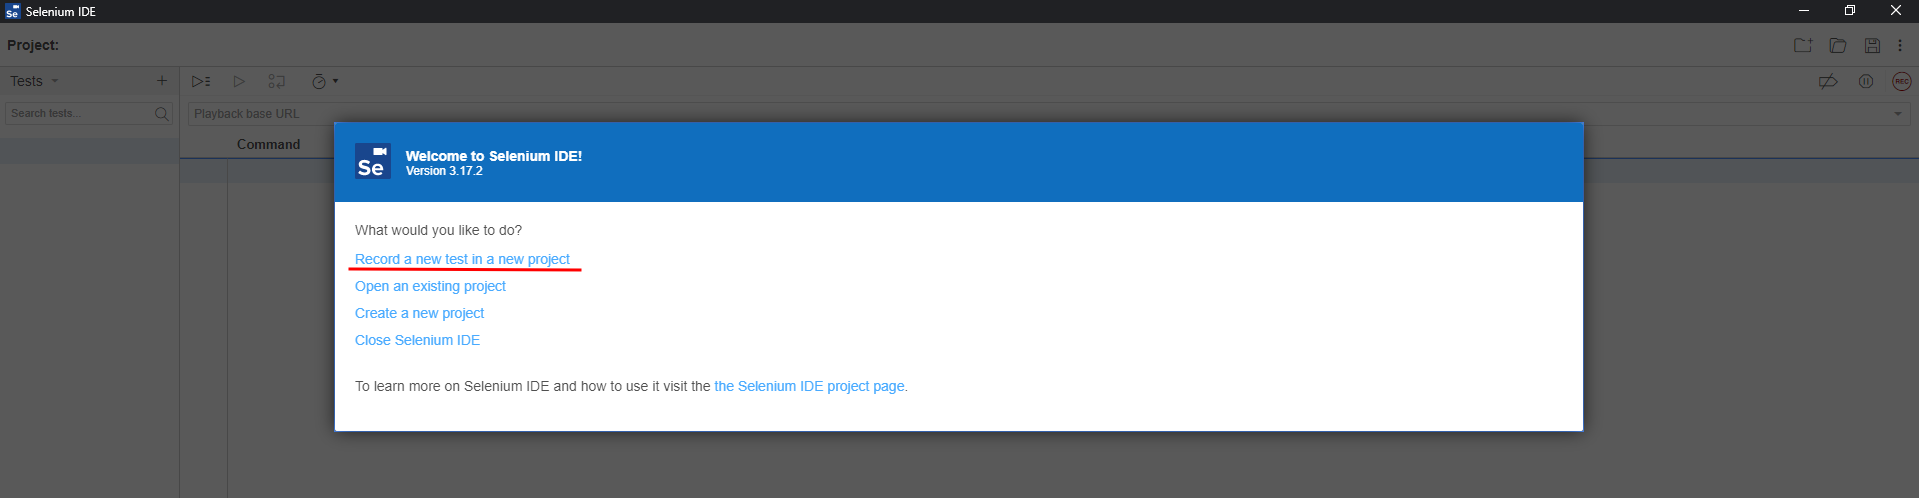
\includegraphics[width=1\textwidth]{seleniumide1}
	\label{fig:seleniumide1}
\end{figure}

\begin{figure}[H]
	\centering
	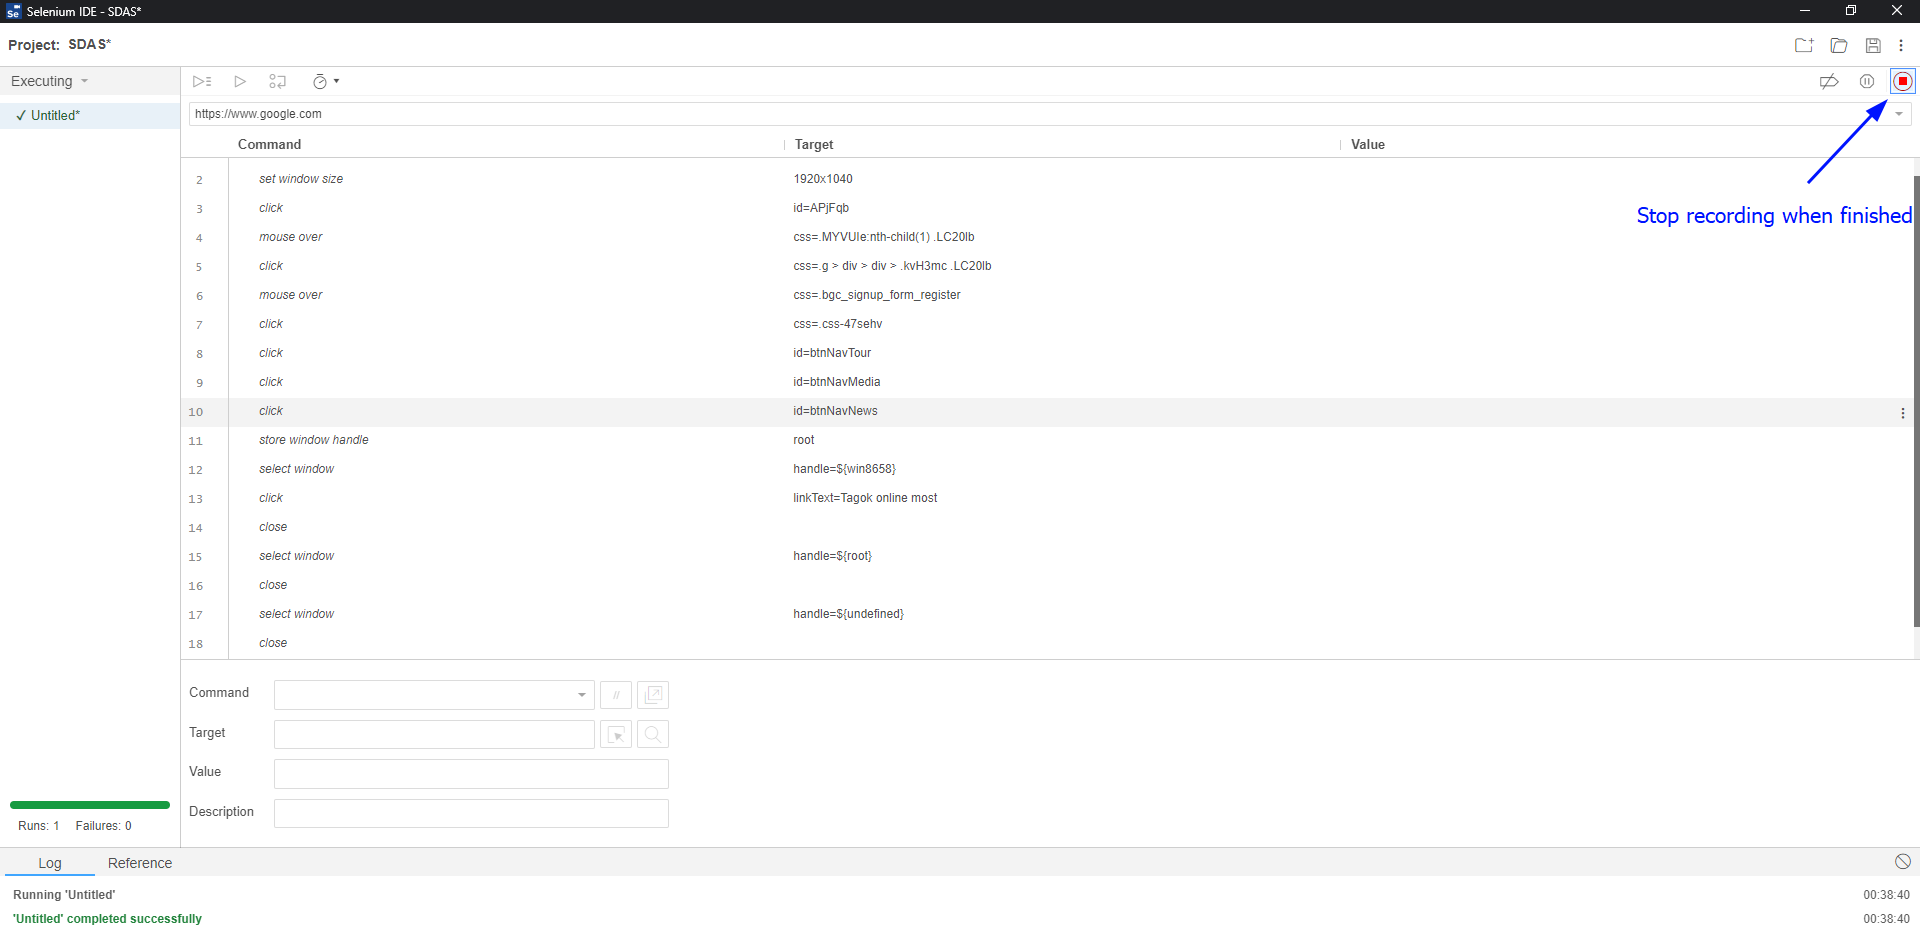
\includegraphics[width=1\textwidth]{seleniumide2}
	\label{fig:seleniumide2}
\end{figure}

Replacing the actions' default target variables with a specific XPath target is advised to increase test reliability. Recommend doing this while utilizing the "XPath Helper" browser plugin and the browsers' inspect mode:

\begin{figure}[H]
	\centering
	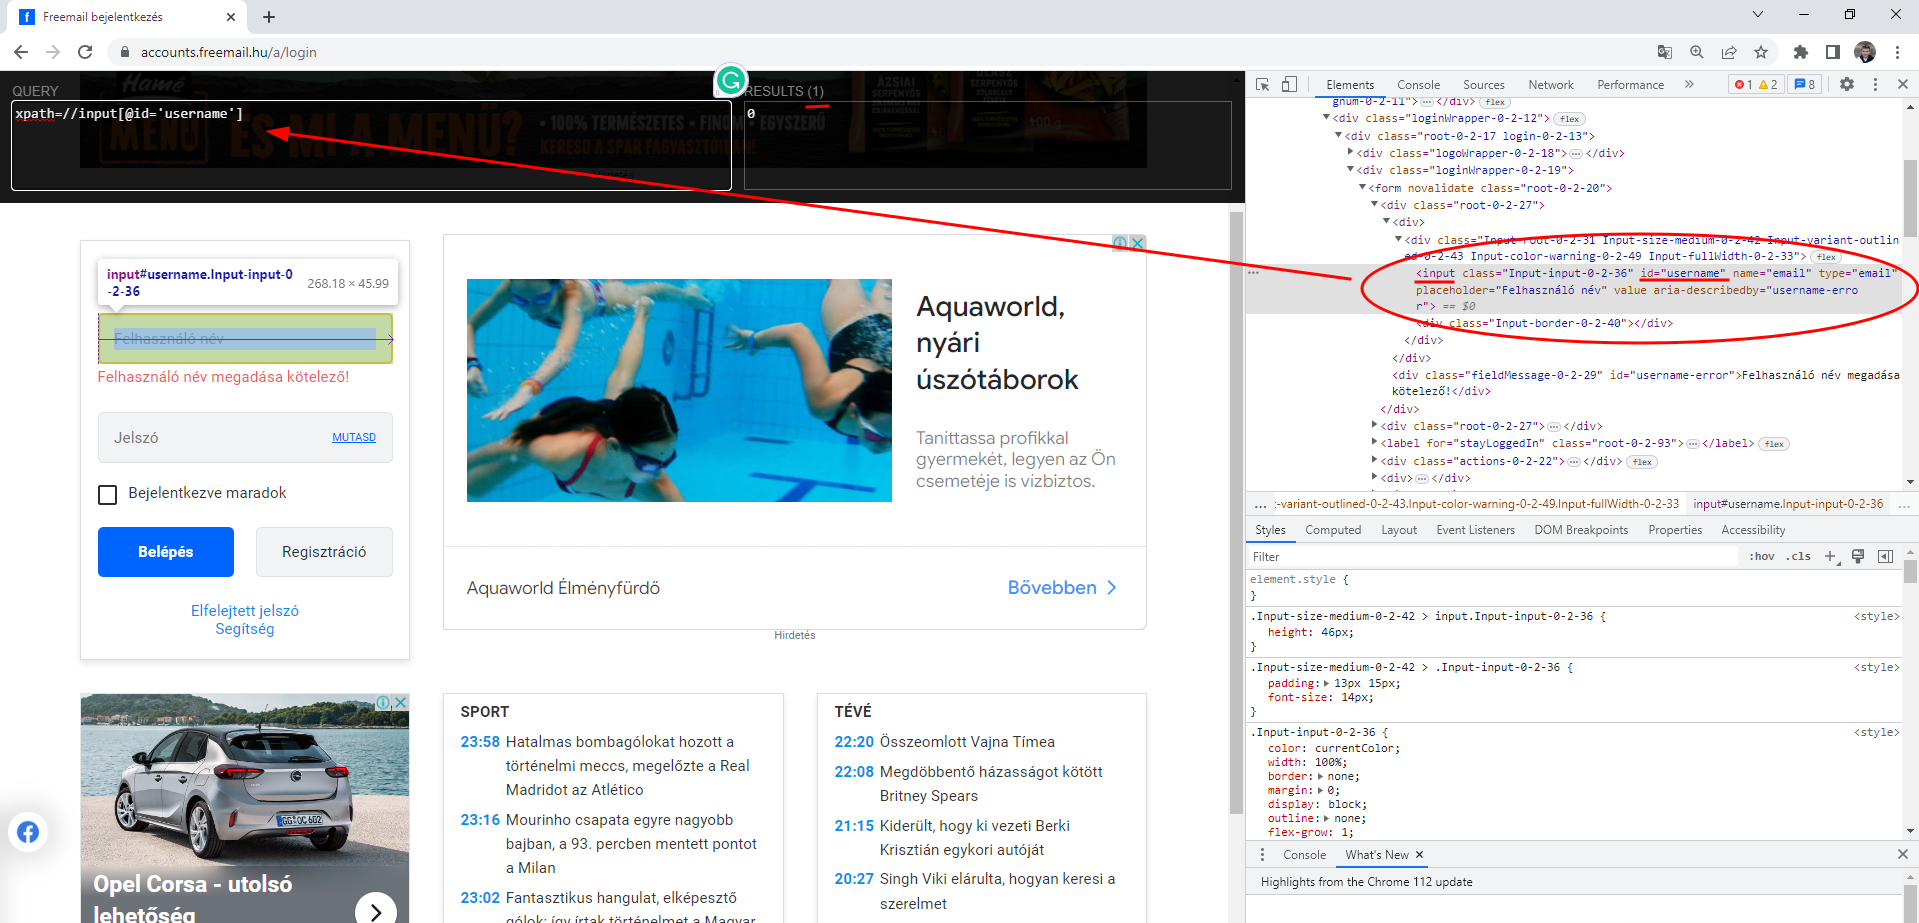
\includegraphics[width=1\textwidth]{xpathhelper}
	\label{fig:xpathhelper}
\end{figure}

\begin{figure}[H]
	\centering
	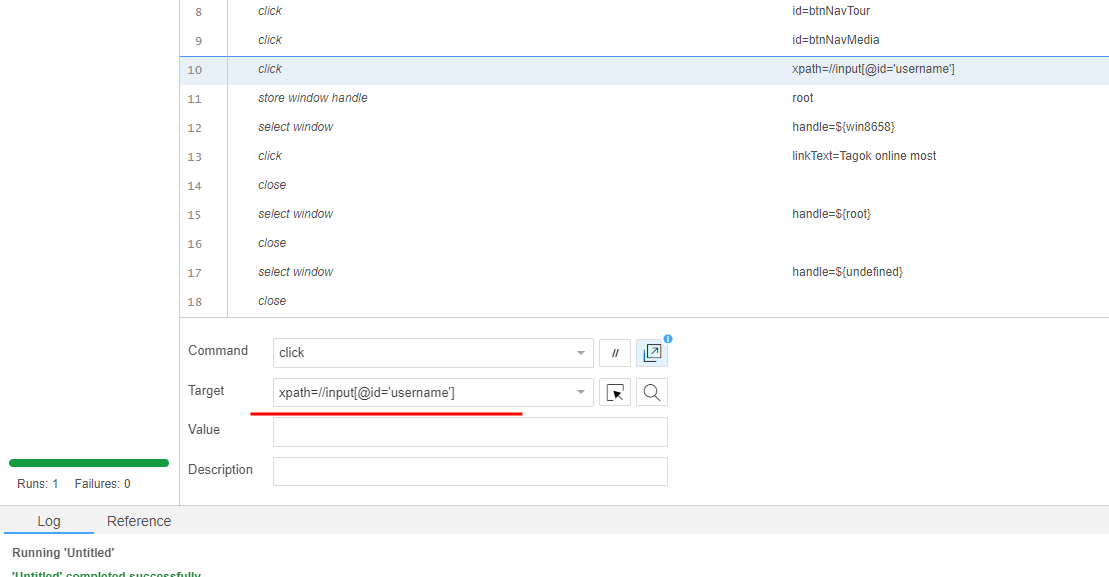
\includegraphics[width=1\textwidth]{seleniumide3}
	\label{fig:seleniumide3}
\end{figure}

Several tests can be conducted within a single test project, and sophisticated Selenium Grid implementations, such as Moon, can perform these tests in a paralyzed fashion to increase efficiency and shorten the testing time. Once finished, save the project into the default .side extension.












\begin{enumerate}
	\item\label{step:first} Donec pretium et quam a cursus. Ut sollicitudin tempus urna et mollis.
	\item Aliquam et aliquam turpis, sed fermentum mauris. Nulla eget ex diam.
	\item Donec eget tellus pharetra, semper neque eget, rutrum diam Step~\ref{step:first}.
\end{enumerate}

Praesent porta, metus eget eleifend consequat, eros ligula eleifend ex, a pellentesque mi est vitae urna. Vivamus turpis nunc, iaculis non leo eget, mattis vulputate tellus. Maecenas rutrum eros sem, pharetra interdum nulla porttitor sit amet. In vitae viverra ante. Maecenas sit amet placerat orci, sed tincidunt velit. Vivamus mattis, enim vel suscipit elementum, quam odio venenatis elit\footnote{Phasellus faucibus varius purus, nec tristique enim porta vitae.}, et mollis nulla nunc a risus. Praesent purus magna, tristique sed lacus sit amet, convallis malesuada magna. 

\begin{description}
	\item[Vestibulum venenatis] malesuada enim, ac auctor erat vestibulum et. Phasellus id purus a leo suscipit accumsan.
	\item[Orci varius natoque] penatibus et magnis dis parturient montes, nascetur ridiculus mus. Nullam interdum rhoncus nisl, vel pharetra arcu euismod sagittis. Vestibulum ac turpis auctor, viverra turpis at, tempus tellus.
	\item[Morbi dignissim] erat ut rutrum aliquet. Nulla eu rutrum urna. Integer non urna at mauris scelerisque rutrum sed non turpis.
\end{description}

\subsection{Lists with narrow spacing inbetween items}

Phasellus ultricies, sapien sit amet ultricies placerat, velit purus viverra ligula, id consequat ipsum odio imperdiet enim:
\begin{compactenum}
	\item Maecenas eget lobortis leo.
	\item Donec eget libero enim.
	\item In eu eros a eros lacinia maximus ullamcorper eget augue.
\end{compactenum}

\bigskip

In quis turpis metus. Proin maximus nibh et massa eleifend, a feugiat augue porta. Sed eget est purus. Duis in placerat leo. Donec pharetra eros nec enim convallis:
\begin{compactitem}
	\item Pellentesque odio lacus.
	\item Maximus ut nisl auctor.
	\item Sagittis vulputate lorem.
\end{compactitem}

\bigskip

Vestibulum ante ipsum primis in faucibus orci luctus et ultrices posuere cubilia Curae; Sed lorem libero, dignissim vitae gravida a, ornare vitae est.
\begin{compactdesc}
	\item[Cras maximus] massa commodo pellentesque viverra.
	\item[Morbi sit] amet ante risus. Aliquam nec sollicitudin mauris
	\item[Ut aliquam rhoncus sapien] luctus viverra arcu iaculis posuere
\end{compactdesc}


\section{Images and figures}

Aliquam vehicula luctus mi a pretium. Nulla quam neque, maximus nec velit in, aliquam mollis tortor. Aliquam erat volutpat. Curabitur vitae laoreet turpis. Integer id diam ligula. Nulla sodales purus id mi consequat, eu venenatis odio pharetra. Cras a arcu quam. Suspendisse augue risus, pulvinar a turpis et, commodo aliquet turpis. Nulla aliquam scelerisque mi eget pharetra. Mauris sed posuere elit, ac lobortis metus. Proin lacinia sit amet diam sed auctor. Nam viverra orci id sapien sollicitudin, a aliquam lacus suscipit, Figure~\ref{fig:example-1}:

\begin{figure}[H]
	\centering
	
\includegraphics[width=0.6\textwidth,height=100px]{elte_cimer_szines}
	\caption{Quisque ac tincidunt leo}
	\label{fig:example-1}
\end{figure}

\subsection{Framing figures}

Ut aliquet nec neque eget fermentum. Cras volutpat tellus sed placerat elementum. Quisque neque dui, consectetur nec finibus eget, blandit id purus. Nam eget ipsum non nunc placerat interdum.

\begin{figure}[H]
	\centering
	
\includegraphics[width=0.6\textwidth,height=100px,frame]{elte_cimer_szines}
	\caption{Quisque ac tincidunt leo}
\end{figure}

\subsection{Subfigures}

In non ipsum fermentum urna feugiat rutrum a at odio. Pellentesque habitant morbi tristique senectus et netus et malesuada fames ac turpis egestas. Nulla tincidunt mattis nisl id suscipit. Sed bibendum ac felis sed volutpat. Nam pharetra nisi nec facilisis faucibus. Aenean tristique nec libero non commodo. Nulla egestas laoreet tempus. Nunc eu aliquet nulla, quis vehicula dui. Proin ac risus sodales, gravida nisi vitae, efficitur neque, Figure~\ref{fig:example-2}:

\begin{figure}[H]
	\centering
	\subcaptionbox{Vestibulum quis mattis urna}{
		
\includegraphics[width=0.45\linewidth]{elte_cimer_szines}}
	\hspace{5pt}
	\subcaptionbox{Donec hendrerit quis dui sit amet venenatis}{
		
\includegraphics[width=0.45\linewidth]{elte_cimer_szines}}
	\caption{Aenean porttitor mi volutpat massa gravida}
	\label{fig:example-2}
\end{figure}

Nam et nunc eget elit tincidunt sollicitudin. Quisque ligula ipsum, tempor vitae tortor ut, commodo rhoncus diam. Pellentesque habitant morbi tristique senectus et netus et malesuada fames ac turpis egestas. Phasellus vehicula quam dui, eu convallis metus porta ac.


\section{Tables}

Nam magna ex, euismod nec interdum sed, sagittis nec leo. Nam blandit massa bibendum mattis tristique. Phasellus tortor ligula, sodales a consectetur vitae, placerat vitae dolor. Aenean consequat in quam ac mollis. 

\begin{table}[H]
	\centering
	\begin{tabular}{ | m{0.25\textwidth} | m{0.65\textwidth} | }
		\hline
		\textbf{Phasellus tortor} & \textbf{Aenean consequat} \\
		\hline \hline
		\emph{Sed malesuada} & Aliquam aliquam velit in convallis ultrices. \\
		\hline
		\emph{Purus sagittis} &  Quisque lobortis eros vitae urna lacinia euismod. \\
		\hline
		\emph{Pellentesque} & Curabitur ac lacus pellentesque, eleifend sem ut, placerat enim. Ut auctor tempor odio ut dapibus. \\
		\hline
	\end{tabular}
	\caption{Maecenas tincidunt non justo quis accumsan}
	\label{tab:example-1}
\end{table}

\subsection{Multi rows and multi columns}

Mauris a dapibus lectus. Vestibulum commodo nibh ante, ut maximus magna eleifend vel. Integer vehicula elit non lacus lacinia, vitae porttitor dolor ultrices. Vivamus gravida faucibus efficitur. Ut non erat quis arcu vehicula lacinia. Nulla felis mauris, laoreet sed malesuada in, euismod et lacus. Aenean at finibus ipsum. Pellentesque dignissim elit sit amet lacus congue vulputate.

\begin{table}[htb]
	\centering
	\begin{tabular}{ | c | r | r | r | r | r | r | }
		\hline
		\multirow{2}{*}{\textbf{Quisque}} & \multicolumn{2}{ c | }{\textbf{Suspendisse}} & \multicolumn{2}{ c | }{\textbf{Aliquam}} & \multicolumn{2}{ c | }{\textbf{Vivamus}} \\
		\cline{2-7}
		& Proin & Nunc & Proin & Nunc & Proin & Nunc \\
		\hline \hline		
		Leo & 2,80 MB & 100\% & 232 KB & 8,09\% & 248 KB & 8,64\% \\
		\hline
		Vel & 9,60 MB & 100\% & 564 KB & 5,74\% & 292 KB & 2,97\% \\
		\hline
		Auge & 78,2 MB & 100\% & 52,3 MB & 66,88\% & 3,22 MB & 4,12\% \\
		\hline 
	\end{tabular}
	\caption[Rövid cím a táblázatjegyzékbe]{Vivamus ac arcu fringilla, fermentum neque sed, interdum erat. Mauris bibendum mauris vitae enim mollis, et eleifend turpis aliquet.}
	\label{tab:example-2}
\end{table}

\subsection{Long tables over multiple pages}

Nunc porta placerat leo, sit amet porttitor dui porta molestie. Aliquam at fermentum mi. Maecenas vitae lorem at leo tincidunt volutpat at nec tortor. Vivamus semper lacus eu diam laoreet congue. Vivamus in ipsum risus. Nulla ullamcorper finibus mauris non aliquet. Vivamus elementum rhoncus ex ut porttitor.

\begin{center}
	\begin{longtable}{ | p{0.3\textwidth} | p{0.7\textwidth} | }
		
		\hline
		\multicolumn{2}{|c|}{\textbf{Praesent aliquam mauris enim}}
		\\ \hline
		
		\emph{Suspendisse potenti} & \emph{Lorem ipsum dolor sit amet}
		\\ \hline \hline
		\endfirsthead % table header on first page
		
		\hline
		\emph{Suspendisse potenti} & \emph{Lorem ipsum dolor sit amet}
		\\ \hline \hline
		\endhead % table header on further pages
		
		\hline
		\endfoot % table footer on previous pages
		
		\endlastfoot % table footer on last page
		
		\emph{Praesent}
		& Nulla ultrices et libero sit amet fringilla. Nunc scelerisque ante tempus sapien placerat convallis.
		\\ \hline
		
		\emph{Luctus}
		& Integer hendrerit erat massa, non hendrerit risus convallis at. Curabitur ultrices, justo in imperdiet condimentum, neque tortor luctus enim, luctus posuere massa erat vitae nibh.
		\\ \hline
		
		\emph{Egestas}
		& Duis fermentum feugiat augue in blandit. Mauris a tempor felis. Pellentesque ultricies tristique dignissim. Pellentesque aliquam semper tristique. Nam nec egestas dolor. Vestibulum id elit quis enim fringilla tempor eu a mauris. Aliquam vitae lacus tellus. Phasellus mauris lectus, aliquam id leo eget, auctor dapibus magna. Fusce lacinia felis ac elit luctus luctus.
		\\ \hline
		
		\emph{Dignissim}
		& Praesent aliquam mauris enim, vestibulum posuere massa facilisis in. Suspendisse potenti. Nam quam purus, rutrum eu augue ut, varius vehicula tellus. Fusce dui diam, aliquet sit amet eros at, sollicitudin facilisis quam. Phasellus tempor metus vel augue gravida pretium. Proin aliquam aliquam blandit. Nulla id tempus mi. Fusce in aliquam tortor.
		\\ \hline
		
		\emph{Pellentesque}
		& Donec felis nibh, imperdiet a arcu non, vehicula gravida nibh. Quisque interdum sapien eu massa commodo, ac elementum felis faucibus.
		\\ \hline
		
		\emph{Molestie}
		& Cras ullamcorper tellus et auctor ultricies. Maecenas tincidunt euismod lectus nec venenatis. Suspendisse potenti. Pellentesque pretium nunc ut euismod cursus. Nam venenatis condimentum quam. Curabitur suscipit efficitur aliquet. Interdum et malesuada fames ac ante ipsum primis in faucibus.
		\\ \hline
		
		\emph{Vivamus semper}
		& In purus purus, faucibus eu libero vulputate, tristique sodales nunc. Nulla ut gravida dolor. Fusce vel pellentesque mi, vel efficitur eros. Nunc vitae elit tellus. Sed vestibulum auctor consequat. 
		\\ \hline
		
		\emph{Condimentum}
		& Nulla scelerisque, leo et facilisis pretium, risus enim cursus turpis, eu suscipit ipsum ipsum in mauris. Praesent eget pulvinar ipsum, suscipit interdum nunc. Nam varius massa ut justo ullamcorper sollicitudin. Vivamus facilisis suscipit neque, eu fermentum risus. Ut at mi mauris.
		\\ \hline
		
		\caption{Praesent ullamcorper consequat tellus ut eleifend}
		\label{tab:example-3}		
	\end{longtable}
\end{center}